\chapter{Zustandsstabilisierung}
\label{Zustandsstabilisierung}

In diesem Kapitel ist die Stabilisierung einer Ruhelage mithilfe der Zustandsrückführung beschrieben. \newline
Bisher wurde nur die Einzelgelenkregelung besprochen. Dabei hat die Regelabweichung eines Gelenkes nur Auswirkungen auf die Stellgröße des Selbigen. Die Matrix $\vect{K_{\mathrm{Regler}}}$ des Reglers hat nur Einträge auf der Diagonalen. Bei der im folgenden beschriebenen Zustandsrückführung kann jeder Zustand, bzw. jede Regelabweichung, die Stellgröße beeinflussen. Dabei ist die Matrix des Reglers theoretisch vollständig besetzt.  

\section{Berechnung der Zustandsrückführung}

Die Zustandsrückführung $\vect{F}$  kann auch als Regler aufgefasst werden, der die Strecke, d.h. das Modell der Betonpumpe, stabilisieren soll. Die Eingänge der Rückführung sind die Zustandsgrößen $\vect{\theta}$, $\vectd{\theta}$, die Winkel und Winkelgeschwindigkeiten der Gelenke und die Parameter der Ruhelage $\vect{\theta}^\mathrm{e}$. Die Stellgröße der Zustandsrückführung wird mit der Stellgröße der Vorsteuerung, wie in Abbildung \ref{fig:Blockdiagramm_Zustandsruckfuhrung} dargestellt, addiert und fungiert als Eingang der Strecke. Die Vorsteuerung berechnet aus dem Arbeitspunkt $\vect{\theta}^\mathrm{e}$, $\vectd{\theta}^\mathrm{e}$, $\vectdd{\theta}^\mathrm{e}$ die konstante Stellgröße zum Halten der Ruhelage. 

	\begin{figure}[h!]
		\centering
		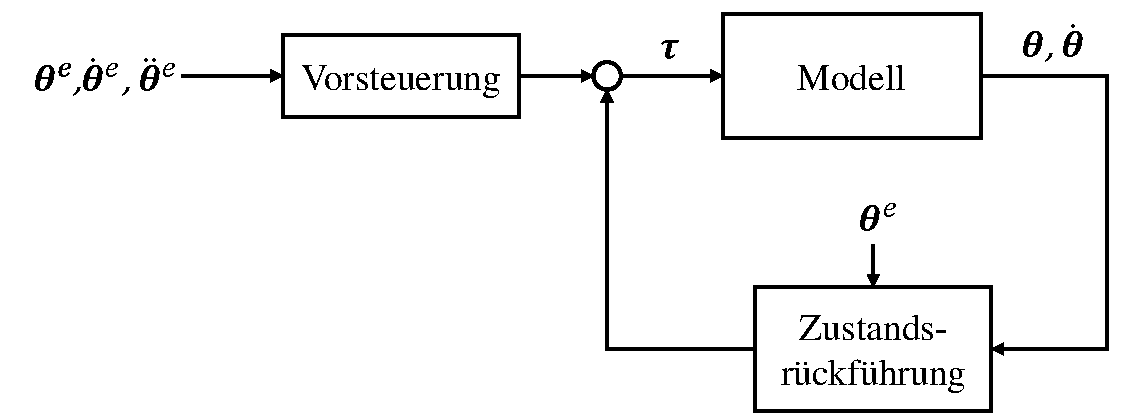
\includegraphics[scale=0.6]{Bilder/Zustansrueckfuehrung.pdf}
		\caption{Blockdiagramm der Zustandsrückführung}
		\label{fig:Blockdiagramm_Zustandsruckfuhrung}
	\end{figure}
	
Die Zustandsrückführung lässt sich aus der Systemmatrix $\vect{A}$, der Eingangsmatrix $\vect{B}$ und den gewünschten Eigenwerten  $\vect{\lambda}$ des Gesamtsystems, das bedeutet Strecke mit Rückführung, berechnen. Dies kann beispielsweise mit der Ackermannformel für Mehrgrößensysteme geschehen. Da das System dafür aufwendig in die Regelungsnormalform überführt werden muss, wird in dieser Arbeit die Rückführung lediglich mit einer bereits existierenden Matlab-Funktion "`place()"' berechnet. 
	
	\begin{equation}
		\vect{F} = \text{place}(\vect{A},\vect{B},\vect{\lambda})
	\end{equation}   	 

Dabei wird die Zustandsrückführung einmalig in Matlab berechnet und nach Python übertragen. Bei sich ständig ändernden Ruhelagen ist diese Vorgehensweise jedoch keine Lösung. Dafür sollte eine Berechnung in Python selbst bevorzugt werden. Zusätzlich kann nicht immer gewährleistet werden, dass die existierenden Algorithmen unter Python oder Matlab eine Lösung liefern. Sie sind abhängig von den gewünschten Eigenwerten, die im nächsten Abschnitt genauer erläutert werden. Es bietet sich daher an, bei veränderlichen Ruhelagen einen eigenen Algorithmus für die Berechnung zu entwickeln.

\section{Polvorgabe}
\label{abs:Polvorgabe}

Aus dem vorangegangen Abschnitt ist ersichtlich, dass die Pole des Gesamtsystems berechnet werden müssen. Sie beschreiben das Verhalten des Systems, welches sich aus der Strecke und der Zustandsrückführung zusammensetzt.\newline
Für den Vergleich werden zuerst die Pole des Systems mit der Einzelgelenkregelung berechnet. Die Eigenwerte des Gesamtsystems lassen sich aus $\vect{A} \in \mathbb{R}^{8\times8}$, $\vect{B} \in \mathbb{R}^{8\times2}$ und $\vect{K_{\mathrm{Regler}}} \in \mathbb{R}^{2\times8}$  mit der Python-Funktion "`np.linalg.eigvals()"' wie folgt berechnen:

	\begin{equation}
		\vect{\lambda} = \text{eig}(\vect{A} + \vect{B} \cdot \vect{K_{\mathrm{Regler}}})
	\end{equation} 

mit:

	\begin{equation*}
		\vect{K_{\mathrm{Regler}}} = \begin{pmatrix}
								3\cdot10^7 & 0 & 0 & 0 & 2\cdot10^7 & 0 & 0 & 0 \\ 
								0 & 0 & 6\cdot10^7 & 0 & 0 & 0 & 3\cdot10^7 & 0
							\end{pmatrix}. 
	\end{equation*} \newline

Es ergeben sich acht Pole, von denen sechs in dem Polplan in Abbildung \ref{fig:Polplan} als blaue Markierungen dargestellt sind. Alle Pole liegen auf der negativen reellen Halbebene. Das System ist somit stabil.  Der eine sichtbare Pol auf der reellen Achse hat eine Vielfachheit von zwei. Zwei der acht Pole sind rein reell mit einem sehr großen Betrag und daher in dem Diagramm nicht abgebildet. \newline
Ausgehend von der Einzelgelenkregelung werden, wie in Abbildung \ref{fig:Polplan} als grüne Markierungen dargestellt, die Pole der "`Polplatzierung 1"' gewählt. Die Beträge der Pole wurden verkleinert, um kleinere Stellsignale zu erhalten. Zusätzlich  wurde der Realteil der Pole, welche nahe an der imaginären Achse lagen, vergrößert. Bei Parameterschwankungen oder einer Regelung geringfügig außerhalb der Ruhelage können sich die Pole des Gesamtsystems verschieben. Liegen die Pole weiter links in der reellen negativen Halbebene kann die Stabilität somit auch bei größeren Schwankungen gewährleistet werden.\newline
Bei der "`Polplatzierung 2"', siehe Abbildung \ref{fig:Polplan} rote Markierungen, wurden sechs statt wie bisher vier der acht Pole konjugiert-komplex gewählt. Des Weiteren sind sie auf einem Kreisbogen um den Ursprung und mit betragsmäßig größerem Realteil angeordnet. Durch das zusätzliche konjugiert-komplexe Polpaar sollte sich die Dynamik des geschlossenen Systems erhöhen. \newline
	
	\begin{figure}[h!]
		\centering
		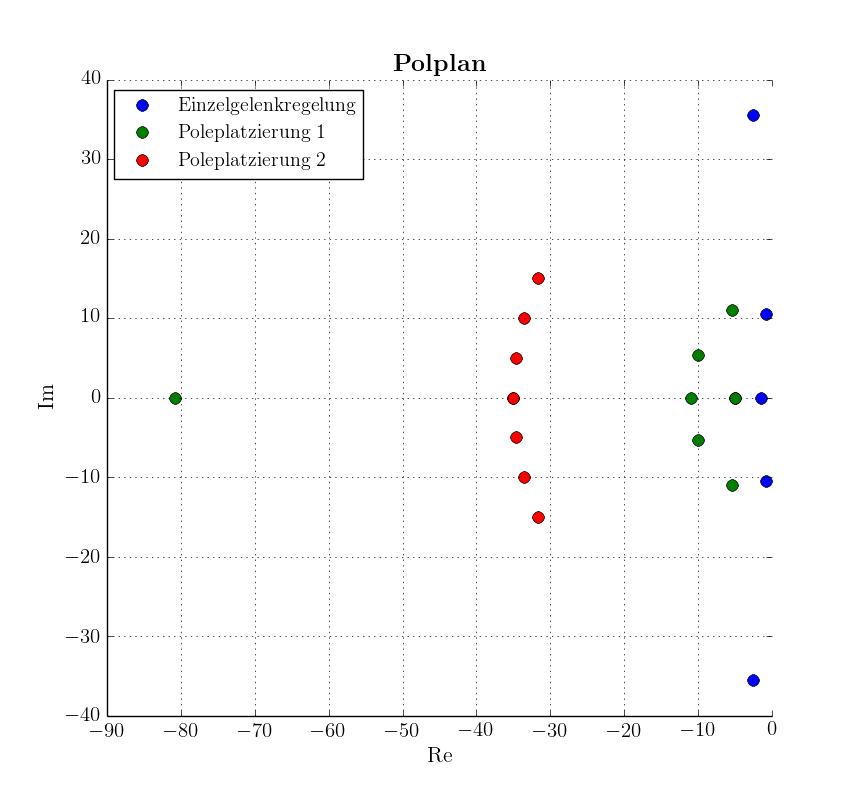
\includegraphics[scale=0.5]{Bilder/Pole.png}
		\caption{Polplan des geschlossenen Kreises}
		\label{fig:Polplan}
	\end{figure}
	
Da sich bei der Polvorgabe in diesem Abschnitt keine eindeutige Lösung finden lässt, sollen im Folgenden die einzelnen Regelungen bzw. Zustandsrückführungen miteinander verglichen werden.

\section{Simulationsergebnisse}

Für den Vergleich der einzelnen Rückführungen belastet man das nichtlineare Modell der Betonpumpe mit einer impulsweise konstanten Last. Diese Art der Belastung entspricht näherungsweise einem realen Pumpvorgang und wurde in Kapitel \ref{abs:Lastmodellierung} beschrieben. Dabei wird die Strecke alle zwei Sekunden für $0,5\,\si{s}$ mit einer zusätzlichen Masse von $100\,\si{kg}$ belastet. Dabei bewegen sich die Gelenke aus der Ruhelage. Die Regelung hat die Aufgabe das System  möglichst schnell, ohne bleibe Regelabweichung und mit geringen Überschwingen in die Ruhelage zu überführen. \newline
Je nach Anwendungsart der Betonpumpe ist die Einhaltung der drei Bedingungen unterschiedlich wichtig. Soll sie beispielsweise in engen und/ oder geschlossenen Räumen manövrieren, darf kein großes Überschwingen auftreten. Wird sie im Freien eingesetzt, spielt das Überschwingen keine große Rolle, hier sollte die Abweichung möglichst schnell ausgeregelt werden. \newline
Die Ergebnisse der Einzelgelenkregelung und der beiden Polplatzierungen aus \mbox{Abschnitt \ref{abs:Polvorgabe}} sind in den folgenden Diagrammen in Abbildung \ref{fig:Ergebnis_Zustandsruckfuhrung} dargestellt. Es sind jeweils die Winkel der aktuierten Gelenke  $\varphi_1 = \theta_{11}$, $\varphi_3 = \theta_{21}$ und die unaktuierten Gelenke $\varphi_2 = \theta_{12}$, $\varphi_4 = \theta_{22}$ über der Zeit $t$ abgebildet. Die Ruhelagen der aktuierten Gelenke betragen $\bar{\varphi}_1 = 60 \,^\circ$, $\bar{\varphi}_3 = -90\,^\circ$. Der Arbeitspunkt der unaktuierten Gelenke wird bei $\bar{\varphi}_2 = \bar{\varphi}_4 = 0 \,^\circ$ angenommen. Aufgrund der Durchbiegung weicht die tatsächliche von der angenommen Ruhelage ab.\newline
Aufgrund dieser Annahme berechnet die Vorsteuerung eine nicht ganz korrekte Stellgröße. Die Regelung versucht am Anfang der Simulation, zwischen $t\in[0;0,5]\,\si{s}$, die  Differenz zu kompensieren. Man erkennt, dass die Zustandsrückführung mit den sechs konjugiert-komplexen Eigenwerten (Polplatzierung 2) sehr schnell mit relativ großen Überschwingen reagiert. Der Stelleingriff an den aktuierten Gelenken hat auch einen Einfluss auf die Unaktuierten.   
    
	\begin{figure}[h!]
		\centering
		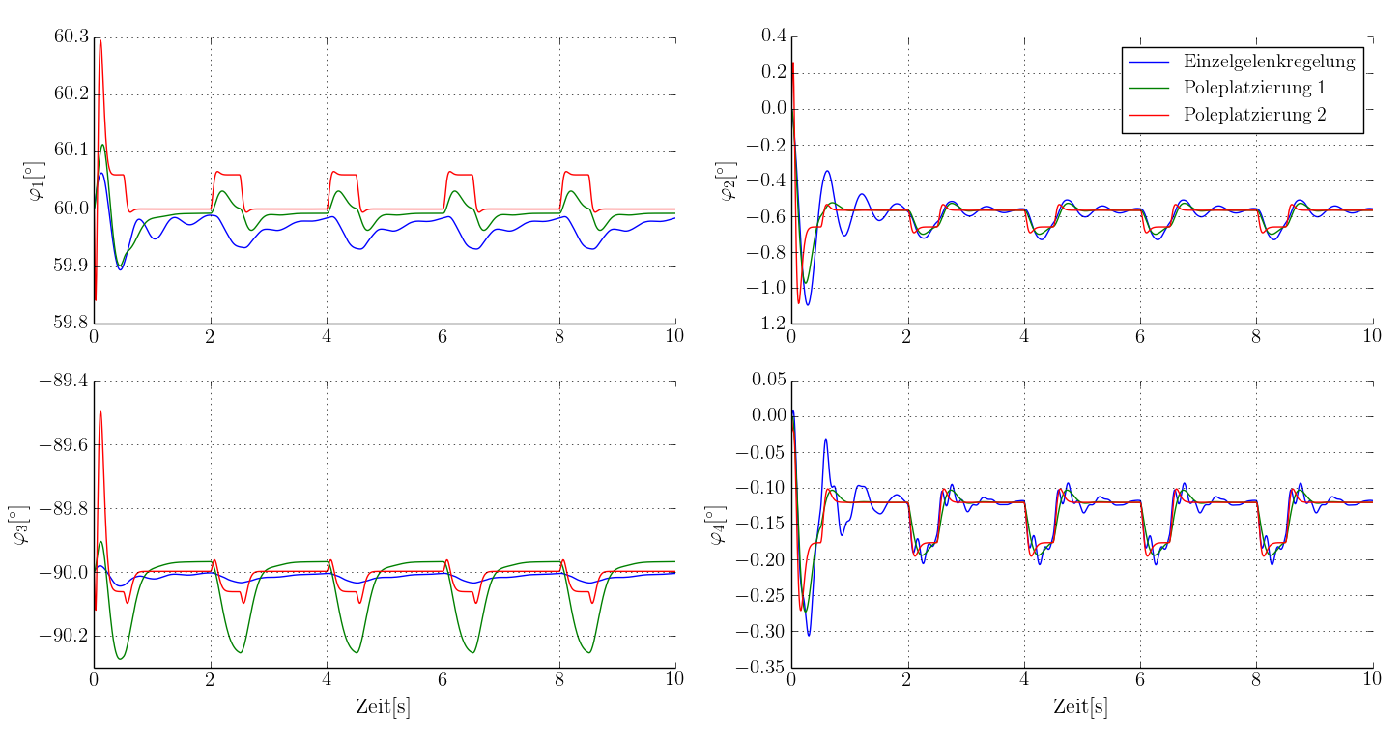
\includegraphics[scale=0.65]{Bilder/Ergebnissse_Zustandsrueckfuehrung.pdf}
		\caption{Verhalten der Zustandsrückführungen bei impulsweiser Belastung}
		\label{fig:Ergebnis_Zustandsruckfuhrung}
	\end{figure}

Die Einzelgelenkregelung schafft es nicht den Fehler der impulsweisen Belastung bei $\varphi_1$ innerhalb der 0,5 s auszuregeln. Auch nach der Entlastung wird der Winkel nur sehr langsam in die Ruhelage gebracht. Ein ähnliches Verhalten ist auch bei dem Gelenk  $\varphi_3$ zu beobachten. Die träge Regelung spiegelt sich auch bei den Winkelverläufen der unaktuierten Gelenke wieder. Bei dem Verlauf von $\varphi_4$ kann man die gewünschten unterschiedlichen Systemfrequenzen aus dem Abschnitt \ref{abs:Federparameter} beobachten.\newline
Die Zustandsrückführung der "`Polplatzierung 1"' in Abbildung \ref{fig:Ergebnis_Zustandsruckfuhrung} weist, wie zu erwarten, eine ähnliche Dynamik wie die Einzelgelenkregelung auf. Lediglich das Überschwingen ist bei $\varphi_1$ verringert. Die Regelung von Gelenk $\varphi_3$ ist dagegen um einiges schlechter. Hier tritt ein größeres Überschwingen bei bleibender Regelabweichung auf. \newline
Wie erwartet weist die Zustandsrückführung der "`Polplatzierung 2"' die größte Dynamik auf. Man erkennt in Abbildung \ref{fig:Ergebnis_Zustandsruckfuhrung}, bei dem Verlauf von $\varphi_1$, dass das System sehr schnell in einen Ruhepunkt überführt wird. Es tritt kaum Überschwingen auf. Während der Belastung wird das System jedoch um eine andere Ruhelage stabilisiert, d.h. es tritt eine bleibende Regelabweichung auf. Ein sehr ähnliches Verhalten zeigt sich auch bei der Regelung von Gelenk $\varphi_3$.\newline
Abschließend lässt sich sagen, dass die Zustandsrückführung der "`Polplatzierung 2"' die besten Ergebnisse liefert. Es würde sich anbieten die Realteile der Pole noch weiter zu erhöhen, um die bleibende Regelabweichung zu verringern. Auch die "`Polplatzierung 1"' liefert für das Gelenk $\varphi_1$ gute Ergebnisse. Es zeigt sich somit, dass bei gut gewählten Polen das System um einiges besser geregelt werden kann als mit der Einzelgelenkregelung. Lediglich das Einstellen der Pole benötigt Erfahrung um das Verhalten des Systems vorauszusagen. 

\chapter{Trajektorien-Folgeregelung}
Bis zu dem jetzigen Stand wurde die Betonpumpe lediglich um eine Ruhelage stabilisiert. Es ist jedoch zusätzlich notwendig den Ausleger der Betonpumpe von einem Arbeitspunkt in einen Anderen zu manövrieren. Die Planung, Steuerung und Regelung des Arbeitspunktwechsel soll im Folgenden näher beschrieben werden. 
\section{Trajektoriengenerierung}
Für den Arbeitspunktwechsel muss eine Trajektorie zwischen den Ruhelagen, im Gelenk\-raum, geplant werden. Diese soll für die Winkel, Winkelgeschwindigkeiten und -beschleuni\-gungen differentiell stetig und glatt sein. \newline
	\begin{figure}[h!]
		\centering
		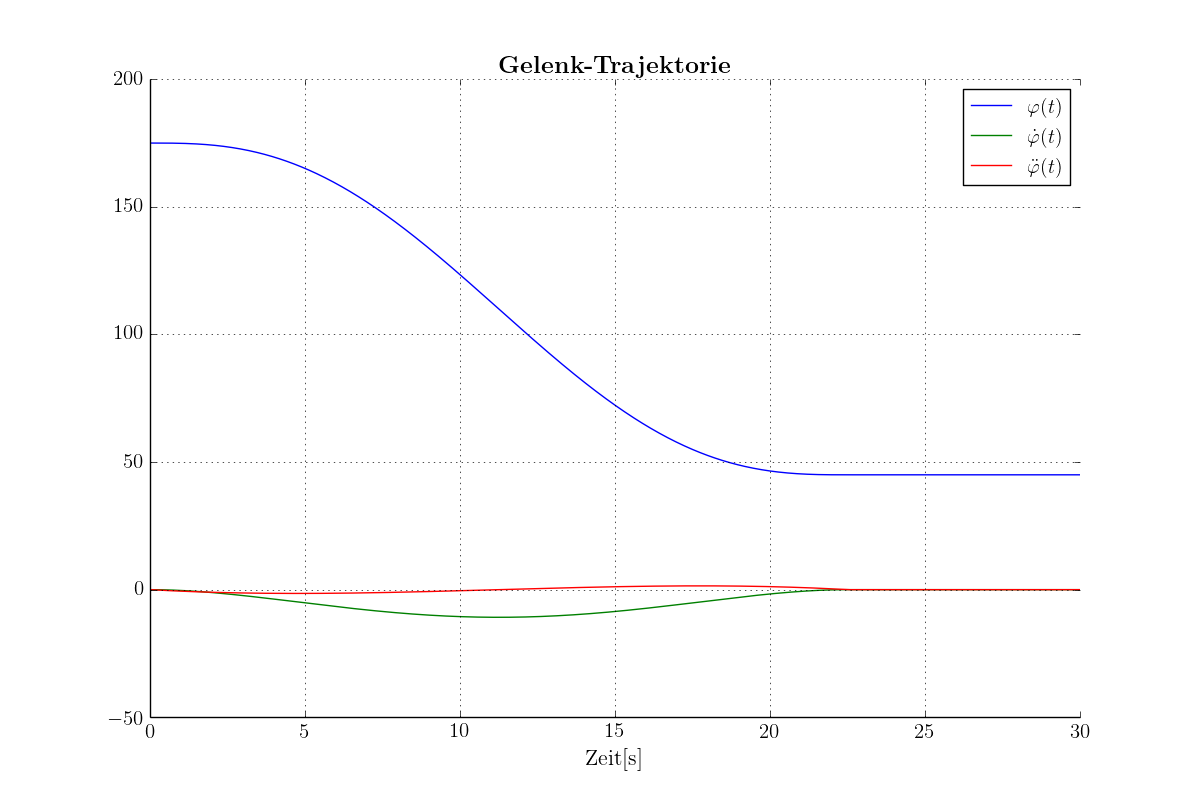
\includegraphics[scale=0.47]{Bilder/Trajektoriengenerierung.png}
		\caption{Beispieltrajektorie für den Arbeitspunktwechsel}
		\label{fig:Trajektoriengenerierung}
	\end{figure}\newline
Es wird ein Polynom vom Grad fünf für die Trajektorie angenommen. Durch Differentiation ergibt sich ein Polynomgrad von drei für die Winkelbeschleunigung. Ein solches Polynom ist stetig differenzierbar und differentiell glatt an den Anfangs- und Endwerten. Die sich daraus ergebenden sechs Unbekannten lassen sich aus den sechs Anfangs- und Endbedingungen und deren Zeiten berechnen. Die Winkelgeschwindigkeiten und -beschleunigungen sind in den Arbeitspunkten null. Die Winkel selbst sind von der Ausgangs- $(\varphi_a)$ und der Ziel- Ruhelage $(\varphi_e)$ abhängig.\newline
Für $\varphi_a= 180\,^\circ$, $\varphi_e= 45\,^\circ$ und einer Zeit $\Delta t=22\,\si{s}$ ergibt sich der in Abbildung \ref{fig:Trajektoriengenerierung} dargestellte Trajektorienverlauf.\newline	 
Da der Arbeitspunktwechsel im Gelenkraum geplant wird, kann wie oben beschrieben, eine separate Trajektorie für jedes Gelenk berechnet werden.\newline
In diesem Projekt wird dafür die bereits vorhandene Funktion "`trans\_poly"' der Bibliotheksklasse "`symb\_tools"' verwendet. Dabei werden wie oben beschrieben, die Anfangs- und Endbedingungen inkl. ihrer Zeitpunkte übergeben.\newline
Die beschriebene Planung der Trajektorie wird in den folgenden Abschnitten als Trajektoriengenerator zusammengefasst. Dieser berechnet zu diskreten Zeitpunkten für alle aktuierten Gelenke ihre Sollwinkel,-geschwindigkeiten und -beschleunigungen .  	
\section{Allgemeiner Aufbau}
Fügt man den neuen Block Trajektoriengenerator in den bereits existierenden Regelkreis mit Vorsteuerung und Einzelgelenkregelung, erhält man das Blockschaltbild aus Abbildung \ref{fig:Blockdiagramm_Trajektorien_Folgeregelung}. \newline
	\begin{figure}[h!]
		\centering
		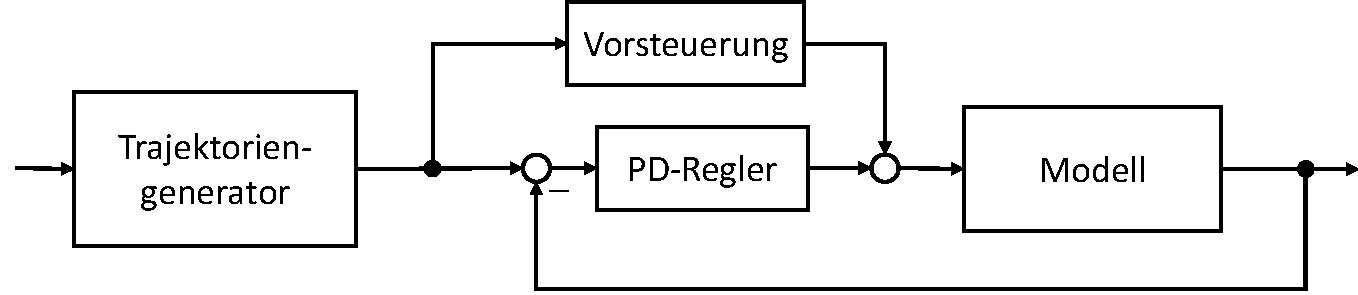
\includegraphics[scale=0.7]{Bilder/Blockdiagramm_Trajektorien_Folgeregelung.pdf}
		\caption{Blockdiagramm der Trajektorien-Folgeregelung}
		\label{fig:Blockdiagramm_Trajektorien_Folgeregelung}
	\end{figure}\newline 
Dabei wird aus dem aktuellen und dem neuen Arbeitspunkt eine Trajektorie berechnet. Zu den, für die Simulation notwendigen, Zeitpunkten werden diskrete Sollwerte für den Regelkreis generiert. Für ein besseres Führungsverhalten berechnet die Vorsteuerung aus den Sollwerten ($\varphi$, $\dot{\varphi}$, $\ddot{\varphi}$) Sollmomente für die Gelenke.\newline
Um den Einfluss von Störungen oder Modellunsicherheiten zu minimieren, wird eine PD-Einzelgelenkreglung hinzugefügt. Diese minimiert den Fehler zwischen dem Soll- und den Istverlauf der Strecke. \newline
Das Modell ist in der Realität die Betonpumpe selbst oder während der Simulation ein mathematisches Modell davon. 
\section{Reglereinstellung}
Bei einer exakten Vorsteuerung ist eine Regelung nicht notwendig, da jedoch das exakte Modell der Betonpumpe nicht abgebildet werden kann, kann auch keine exakte Vorsteuerung berechnet werden. So wird beispielsweise angenommen, dass die unaktuierten Gelenke einen konstanten Winkel von $\varphi = 0$ haben, in Wahrheit weichen sie um bis zu einigen Grad davon ab. Eine Regelung ist somit zwingend notwendig. \newline
Zusätzlich handelt es sich um ein hochgradig nichtlineares Modell. Bei der Verwendung der Zustandsstabilisierung aus Kapitel \ref{Zustandsstabilisierung} wäre die Linearisierung und somit die Systemmatrix abhängig von der Zeit, man erhält ein zeitvariantes System. Die Verwendung von nichtlinearen Regelungsansätzen ist ebenfalls kompliziert, da es sich um ein Mehrgrößensystem handelt und kein flacher Ausgang für das System gefunden wurde.\newline
Demzufolge soll in dieser Arbeit die Trajektorie mit einer einfachen PD-Reglung stabilisiert werden. Ein I-Anteil ist nicht notwendig, da die Stellgröße als Moment vorgegeben wird und die Sollgröße ein Winkel ist. Der offener Kreis besitzt somit bereits zwei Integratoren.\newline
	\begin{figure}[h!]
		\centering
		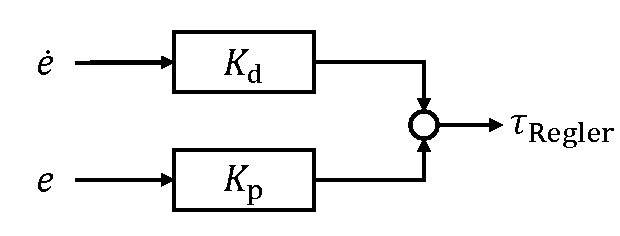
\includegraphics[scale=0.7]{Bilder/PD_Regler.pdf}
		\caption{Blockdiagramm der PD-Regelung}
		\label{fig:Blockdiagramm_PD_Regelung}
	\end{figure}\newline
Die PD-Regelung aus Abbildung \ref{fig:Blockdiagramm_PD_Regelung} wird als Einzelgelenkregler verwendet. In dieser Arbeit werden der Einfachheit halber nur Betonpumpen mit zwei aktuierten Gelenken untersucht. Es müssen somit vier Reglerparameter einzeln eingestellt werden.\newline
Die Parameter werden gleichmäßig erhöht, bis sich ein stabiles Verhalten mit hinreichend geringer Regelabweichung einstellt. Abhängig davon stellt man nun die Verstärkungen unabhängig voneinander ein, bis das gewünschte Verhalten erzielt wird. Dieses Vorgehen kann nur simulativ durchgeführt werden, um die Betonpumpe im Falle von instabilen Verhalten nicht zu beschädigen. Als Qualitätskriterium wird die Regelabweichung nach ca. zehn Sekunden verwendet, welche ungefähr der bleibenden Regelabweichung entspricht. Tabelle \ref{tab:Reglerparameter} zeigt die bleibende Regelabweichung für verschiedene Reglerparameter.\newline
	\begin{table}[h!]
	\caption{PD-Reglerparametrierung}
	\label{tab:Reglerparameter}
	\begin{tabular}{|c|c|c|c|c|c|c|}
		\hline \rule[-2ex]{0pt}{5.5ex}  Regler & $K_{\mathrm{p},1}\:\left[ \frac{\si{Nm}}{\si{rad}}\right]$ & $K_{\mathrm{d},1}\:\left[ \frac{\si{Nm}\cdot\si{s}}{\si{rad}}\right]$ & $K_{\mathrm{p},2}\si{ }\left[ \frac{\si{Nm}}{\si{rad}}\right]$ & $K_{\mathrm{d},2}\:\left[ \frac{\si{Nm}\cdot\si{s}}{\si{rad}}\right]$ & $e_{\varphi_1,\infty}\,^\circ$ & $e_{\varphi_3,\infty}\,^\circ$ \\ 
		\hline \rule[-2ex]{0pt}{5.5ex} $0$ & $1\cdot10^5$  & $1\cdot10^5$ & $1\cdot10^5$ & $1\cdot10^5$ & $-216,8$ & $-60,34$ \\
		\hline \rule[-2ex]{0pt}{5.5ex} $1$ & $1\cdot10^6$  & $1\cdot10^6$ & $1\cdot10^6$ & $1\cdot10^6$ & $6,854\cdot10^{-2}$ & $-1,226\cdot10^{-1}$ \\
		\hline \rule[-2ex]{0pt}{5.5ex} $2$ & $1\cdot10^7$  & $1\cdot10^7$ & $1\cdot10^7$ & $1\cdot10^7$ & $5,467\cdot10^{-3}$ & $-1,248\cdot10^{-2}$ \\
		\hline \rule[-2ex]{0pt}{5.5ex} $3$ & $3\cdot10^7$  & $2\cdot10^7$ & $6\cdot10^7$ & $3\cdot10^7$ & $1,783\cdot10^{-3}$ & $-2,087\cdot10^{-3}$ \\
		\hline 
	\end{tabular} 
	\end{table}
Man erkennt, dass bei zu geringen Verstärkungen (Regler 0) das System instabiles Verhalten aufweist. Erhöht man die Parameter um eine Potenz (Regler 1) stabilisiert der Regler die Strecke. Nun werden die Parameter solange angepasst, bis sich eine Genauigkeit von einigen tausendstel Grad einstellt. Es ergibt sich die Reglerparameterkonstellation drei.\newline
Es ist ersichtlich, dass trotz der zwei Integratoren der Strecke die bleibe Regelabweichung nicht auf Null geregelt werden kann. Eine Genauigkeit von wenigen tausendstel Grad ist jedoch für den Betrieb einer Betonpumpe mehr als ausreichend.
\section{Simulationsergebnisse}
Eine typische Bewegung der Betonpumpe ist in Abbildung \ref{fig:Verlauf_Trajektorienfolgeregelung} dargestellt. Dabei werden die Glieder aus einer Transportposition (alle Glieder sind auf dem Transportfahrzeug eingeklappt, siehe linker Teil) in eine Arbeitsposition (siehe rechter Teil) verfahren. Die in dem Diagramm in Abbildung \ref{fig:Verlauf_Trajektorienfolgeregelung} gezeigten Gelenkverläufe sind die simulierten Verläufe. 
	\begin{figure}[h!]
		\centering
		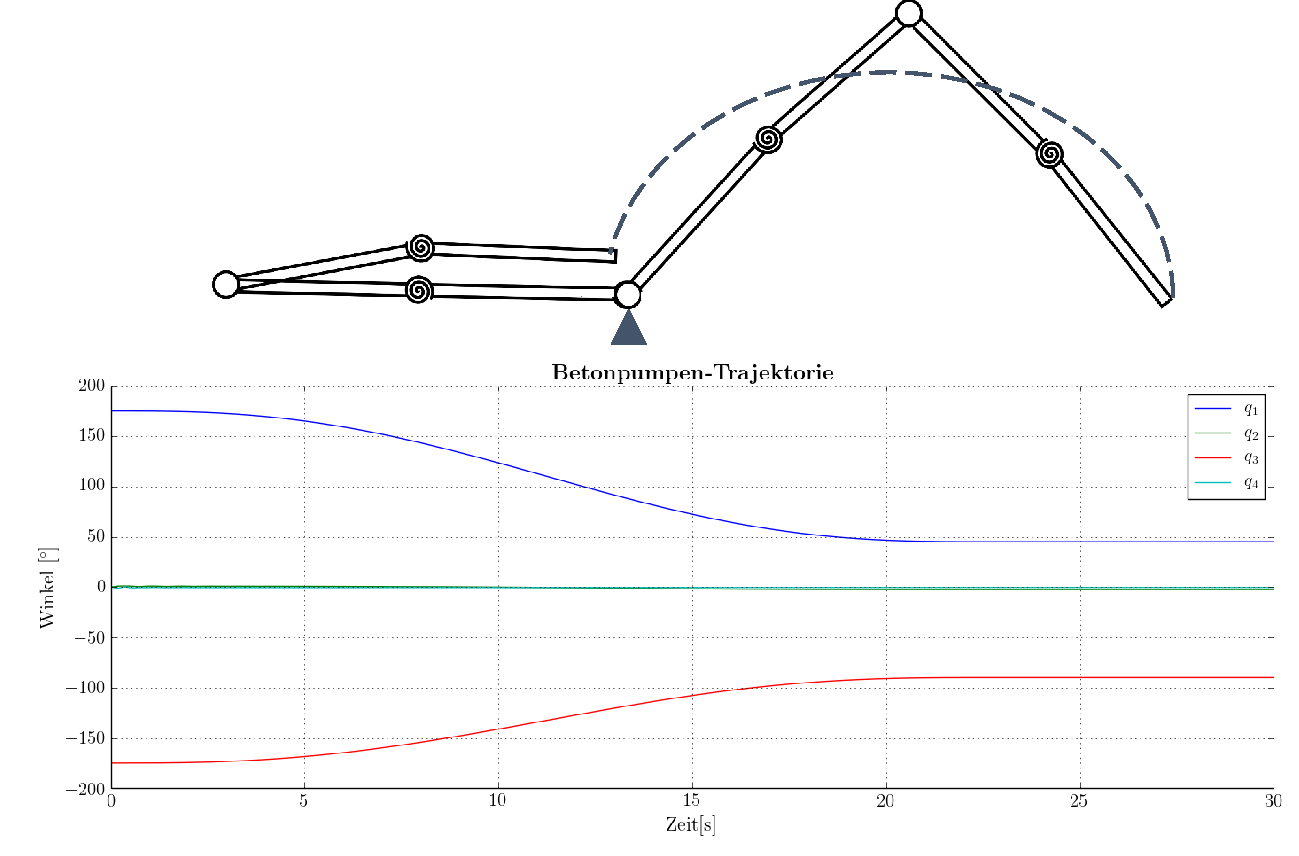
\includegraphics[scale=0.7]{Bilder/Verlauf_Trajektorienfolgeregelung.pdf}
		\caption{Gelenktrajektorien mit Folgeregelung}
		\label{fig:Verlauf_Trajektorienfolgeregelung}
	\end{figure}\newline
Stellt man die Regelabweichungen während der Bewegung der Gelenke $\varphi_1$  und $\varphi_3$ über die Zeit dar, erhält man das Diagramm in Abbildung \ref{fig:Regelabweichung_Folgeregelung}. Die bleibenden Abweichungen aus Tabelle \ref{tab:Reglerparameter} entsprechen den Regelabweichungen bei $t=30\,\si{s}$. Man erkennt, dass die Differenz aus Soll- und Istwinkeln in der Transportposition ($t=3\,\si{s}$) bedeutend kleiner als in der Arbeitsposition ($t=30\,\si{s}$) ist.
\newline 
	\begin{figure}[h!]
		\centering
		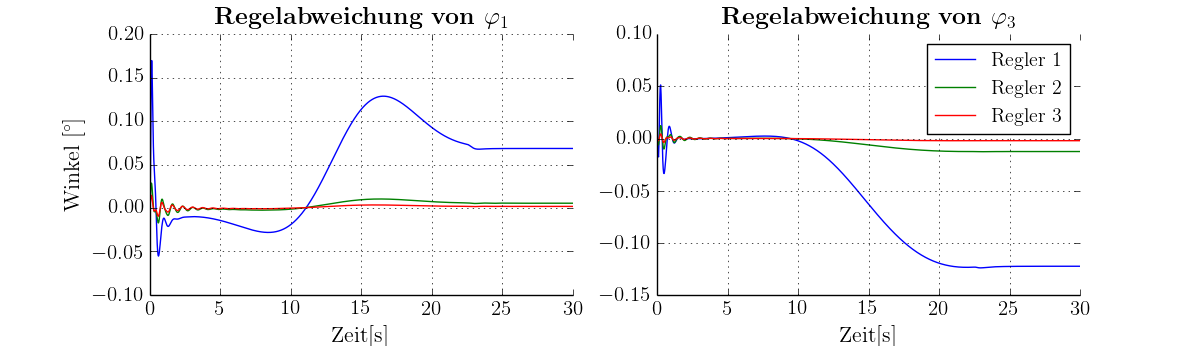
\includegraphics[scale=0.55]{Bilder/Regelabweichung_Folgeregelung.png}
		\caption{Regelabweichung der Trajektorien-Folgeregelung für $\varphi_1$, $\varphi_3$}
		\label{fig:Regelabweichung_Folgeregelung}
	\end{figure}\newline
	
\section{Stellgrößenabschätzung}
Theoretisch wäre es möglich die bleibende Regelabweichungen durch sehr große Verstärkungen immer weiter zu minimieren. Die Stellgrößen hängen jedoch direkt von den Reglerparametern und der Vorsteuerung ab. Daher bietet es sich an im Folgenden eine maximale Schranke für die Stellgrößen zu schätzen. \newline
Für die obere Grenze soll die Betonpumpe vollständig ausgestreckt mit ihrer kompletten Masse am äußersten Punkt belastet werden. Abbildung \ref{fig:Stellgroessenabschaetzung} zeigt diese Anordnung für die in der Arbeit diskutierten Betonpumpe mit jeweils zwei aktuierten und unaktuierten Gelenken.   
\newline
	\begin{figure}[h!]
		\centering
		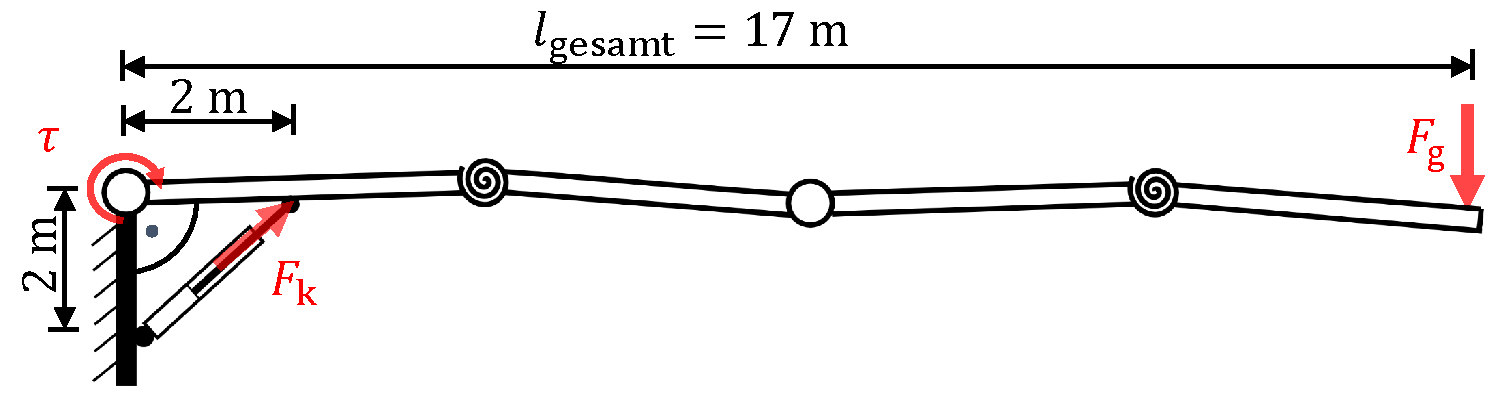
\includegraphics[scale=0.6]{Bilder/Stelgroessenabschaetzung.pdf}
		\caption{Abschätzung der maximalen Stellgrößen}
		\label{fig:Stellgroessenabschaetzung}
	\end{figure}\newline
Durch eine Belastung von $m_{\mathrm{gesamt}} = 4250\,\si{kg}$ ergibt sich ein Moment $\tau_g$ von:
	\begin{equation}
		\tau_g = l_{\mathrm{gesamt}}\cdot g\cdot m_{\mathrm{gesmat}}\approx 700 \,\si{kNm}.
	\end{equation}  
Bei der Verwendung eines trivial angeordneten Hydraulikzylinders, wie in Abbildung \ref{fig:Stellgroessenabschaetzung}, muss eine Kraft $F_k$ aufgebracht werden, um das Moment $\tau_g$ zu kompensieren.  Es gilt:
	\begin{equation}
		\tau = \tau_k-\tau_g = 0 \,\si{Nm}.
	\end{equation}
Somit ergibt sich $F_k$ zu
	\begin{equation}
		F_k = \sqrt{2}\cdot \frac{\tau_k}{2\,\si{m}} \approx 500\,\si{kN}.
	\end{equation}

Recherchen zeigen, dass Kräfte von mehr als $500\,\si{kN}$ mit Hydraulikzylindern realisiert werden können. Aus Sicherheitsgründen wird die Kraft etwas erhöht und eine maximale Stellgröße von $\tau_{k,\mathrm{max}} = 1 \,\si{MNm}$ verwendet. Während der Simulation werden alle Stellgrößen auf diesen Wert beschränkt.\newline
\newline
	\begin{figure}[h!]
		\centering
		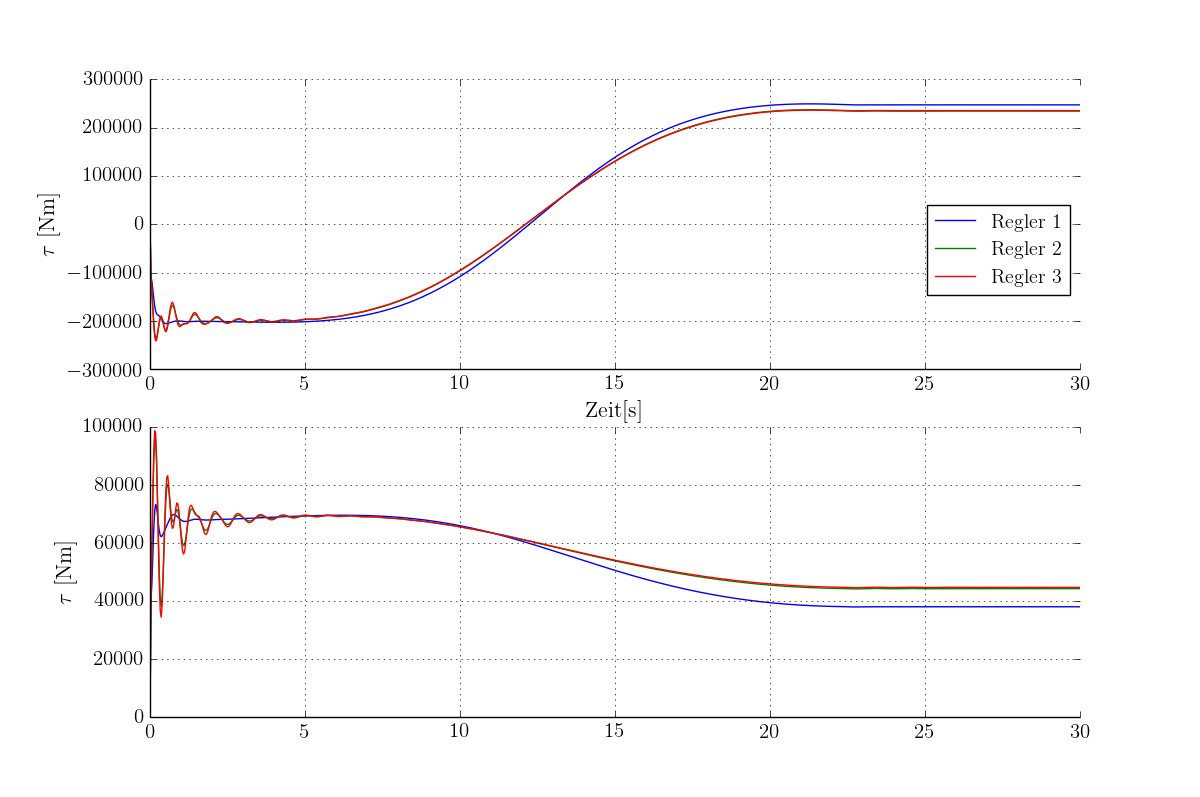
\includegraphics[scale=0.5]{Bilder/Stellgroessen_Trajektorien_Folgeregelung.png}
		\caption{Stellgrößenverlauf der Trajektorien-Folgeregelung}
		\label{fig:Stellgroessen_Trajektorien_Folgeregelung}
	\end{figure}\newline
Der Stellgrößenverlauf der Trajektorien-Folgeregelung ist in Abbildung \ref{fig:Stellgroessen_Trajektorien_Folgeregelung} dargestellt. Man erkennt, dass die maximale Stellgröße von $\tau_{k,\mathrm{max}} = 1 \,\si{MNm}$ weit unterschritten wird. Die Bewegung kann somit von einer realen Betonpumpe durchgeführt werden. 

\section{Einführung von Modellungenauigkeiten}
Aus Abbildung \ref{fig:Stellgroessen_Trajektorien_Folgeregelung} ist ersichtlich, dass die Regelung nach der Einschwingphase, ab $t=5\,\si{s}$ kaum dynamische Stellgrößen generiert. Es zeigt sich, dass die Vorsteuerung sehr gut dem inversen Streckenmodell entspricht. Bei einer realen Betonpumpe wird dies nicht mehr der Fall sein. Um dennoch Stabilität und ein gutes Führungsverhalten gewährleisten zu können, werden nachfolgend Modellungenauigkeiten eingefügt, die nicht in der Vorsteuerung betrachtet werden.\newline
	\begin{figure}[h!]
		\centering
		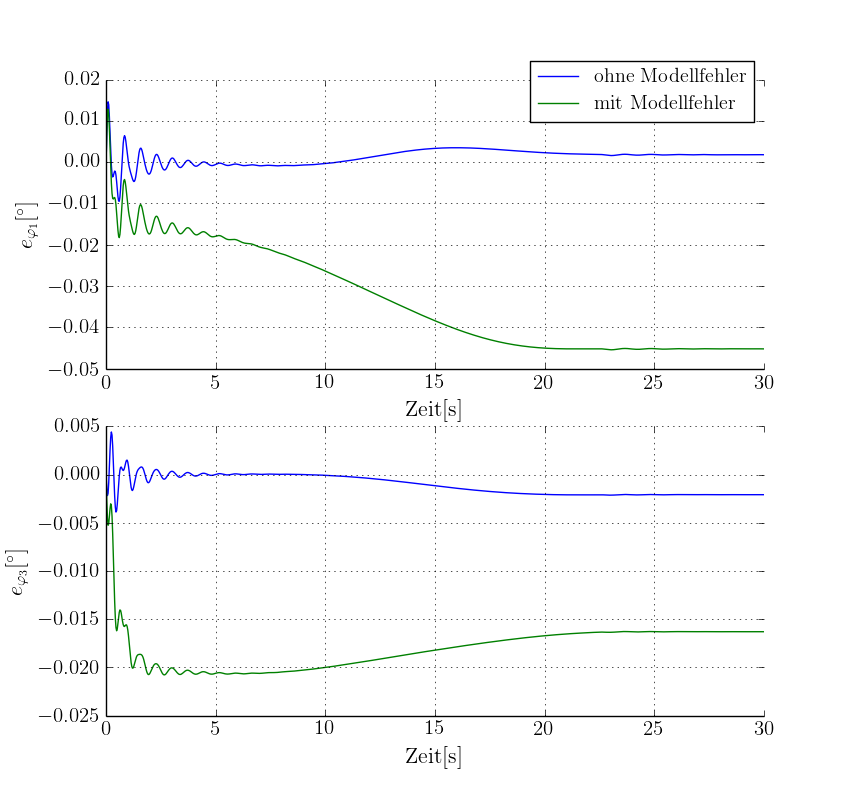
\includegraphics[scale=0.5]{Bilder/Modellungenauigkeiten.png}
		\caption{Regelabweichung mit Modellungenauigkeiten}
		\label{fig:Regelabweichung_Modellungenauigkeiten}
	\end{figure}\newline
Dabei wird der Wert aller Modellparameter für die Simulation um $\pm20 \,\%$ variiert. Abbildung \ref{fig:Regelabweichung_Modellungenauigkeiten} zeigt den Verlauf der Regelabweichung während der Bewegung. Es ist ersichtlich, dass das System trotz der Ungenauigkeiten stabilisiert werden kann. Lediglich die Regelabweichungen sind um einiges größer. Da es sich bei den Ungenauigkeiten um eine zufällige Verteilung handelt werden fünf Messungen durchgeführt und die stationären Regelabweichungen gemittelt. Die ermittelten Werte von \mbox{$e_{\varphi_1,\infty}=4,508\cdot10^{-2}\,^\circ$} und $e_{\varphi_3,\infty} = 5,368\cdot10^{-3}\,^\circ$  liegen jedoch immer noch weit unter den für den Betrieb einer Betonpumpe notwendigen Abweichungen. Diese ersten Versuche zeigen, dass die Trajektorien-Folgeregelung durchaus auch bei einer realen Betonpumpe mit zwei Armsegmenten angewendet werden kann. 

\chapter{Zusammenfassung und Ausblick}
Die hier angefertigte Arbeit ist Teil des Oberseminars der Regelungs- und Steuerungstheorie. Ziel des Seminars war die Untersuchung, Steuerung und Regelung eines Auslegers einer mobilen Betonpumpe. Die Arbeit wurde in einer Gruppe von drei Studenten durchgeführt. Im folgenden Abschnitt werden die Ergebnisse noch einmal zusammengefasst dargestellt und ein Ausblick für das mögliche weitere Vorgehen gegeben
  
\section{Zusammenfassung der Ergebnisse}
Einen großen zeitlichen Aufwand stellte die Darstellung des Verhaltens der Ausleger der Betonpumpe als mathematische Gleichungen dar. Diese Modellierung wurde mit konzentrierten Parametern durchgeführt. Um das dynamische Verhalten und die Durchbiegung gut darstellen zu können, wurde pro Armsegment ein passives unaktuiertes Zusatzgelenk betrachtet. Diese Modellierung war die Voraussetzung für alle weiteren Schritte.\newline
Um das Systemverhalten der Betonpumpe abzubilden, wurden sämtliche Parameter der Modellierung unter Verwendung von realen Daten berechnet. \newline
Zusätzlich wurde das erhaltene Systemmodell linearisiert und in die Zustandsdarstellung überführt. Dadurch war es möglich einen Nachweis der Stabilität in der Ruhelage zu erbringen und eine Zustandsrückführung zu berechnen.\newline
Es wurden verschiedene Varianten diskutiert, wie viele Modellinformationen für die Regelung und Steuerung einbezogen werden sollen. Dadurch konnten ihre Auswirkungen auf das Verhalten der Betonpumpe in mehreren Simulationen untersucht werden.\newline
Es wurde eine impulsweise Belastung eingeführt, die die reale Belastung gut approximiert. Dadurch war es möglich verschiedene Regelungskonzepte miteinander zu vergleichen.\newline
Diese Regelungskonzepte sind u.a. die Einzelgelenkregelung, wo jedes Gelenk unabhängig von den anderen mit einem PD-Regler stabilisiert wird. Als eine weitere Möglichkeit für die Ruhelagenstabilisierung wurde die Zustandsrückführung vorgestellt. Dafür wurden die gewünschten Eigenwerte des Gesamtsystems vorgegeben, um eine Rückführung zu berechnen.\newline
Des Weiteren wurden Trajektorien im Gelenkraum geplant, um den Ausleger der Betonpumpe in eine neue Ruhelage überführen zu können. Die Stabilisierung während der Bewegung übernimmt eine Trajektorien-Folgeregelung. Für ein gutes Verhalten wurden die Parameter der Regelung gezielt eingestellt.\newline 
Letztendlich können durch die Einführung von Modellungenauigkeiten die genannten Konzepte der Regelung und Steuerung auch mit fehlerhaften Systemmodellen getestet werden. Dadurch ist es möglich ihr Verhalten bei einer realen Anwendung besser abschätzen zu können.
\section{Ausblick für weiteres Vorgehen}

Die Zusammenfassung in dem vorherigen Abschnitt zeigt, dass viele verschiedene Möglichkeiten der Modellierung, Regelung und Steuerung des Auslegers einer mobilen Betonpumpe untersucht wurden. Trotzdem konnten im Umfang des Oberseminars nicht alle möglichen Konzepte behandelt werden. \newline
So wurden bisher nur lineare Regelungskonzepte implementiert. Die Kenntnisse über Nichtlinearitäten konnten dabei leider nicht verwendet werden. Eine andere Möglichkeit ist die Eingang-Ausgang-Linearisierung. Dabei wird das vorhandene nichtlineare Modell partiell linearisiert, indem ein neuer Eingang eingeführt wird. Die neue Stellgröße ist die Winkelbeschleunigung. Bisher wurde das Moment als Eingang benutzt. Das daraus entstandene partiell lineare System kann mit den Methoden der linearen Regelungstechnik stabilisiert werden. \newline
Des Weiteren kann eine Trajektorienplanung für die unaktuierten Gelenke entwickelt werden. Da diese Gelenke nicht aktiv gesteuert werden können, beschreibt die Trajektorie nur die Bewegung, die durch die Steuerung der aktuierten Gelenke verursacht wird. Dadurch kann der gesamte Ausleger auf einer gezielten Trajektorie in Gelenk- und Arbeitsraum (Raumkoordinaten und Orientierung) bewegt werden. Bei dieser Aufgabe wird  eine Randwertaufgabe gelöst.\newline
In dieser Arbeit wurden bisher alle Untersuchungen lediglich an einem Ausleger mit zwei aktuierten Gelenken vorgenommen. In der Einleitung erkennt man, dass eine reale Betonpumpe mehr als fünf aktive Gelenke besitzen kann. Es sollten daher die in der Arbeit vorgestellten Konzepte der Regelung und Steuerung auf eine solche Anzahl übertragen werden. Dabei entstehen sehr große Gleichungssysteme, die ein symbolisches Lösen nahezu unmöglich machen.\newline
Trotz der genannten unbearbeiteten Aufgaben bieten die in dieser Arbeit gezeigten Ergebnisse eine gute Grundlage für die tatsächliche Regelung und Steuerung einer mobilen Betonpumpe.
